\documentclass[a4paper,12pt]{article}
\usepackage[russian]{babel}   
\usepackage[utf8]{inputenc}
\usepackage{amssymb}
\usepackage{amsmath}
\usepackage{amsfonts}
\usepackage{enumerate}
\usepackage{titlesec}
\usepackage[left=30mm, top=20mm, right=20mm, bottom=20mm, nohead, footskip=10mm]{geometry} % настройки полей документа
\usepackage{indentfirst}
\usepackage{graphicx}

\graphicspath{{pictures/}}
\DeclareGraphicsExtensions{.png,.jpg}

\newcommand{\sectionbreak}{\clearpage}

\renewcommand{\emptyset}{\varnothing}
\renewcommand{\bar}[1]{\overline{#1}}
\renewcommand{\thesection}{\arabic{section}.}
\renewcommand{\thesubsection}{\arabic{section}.\arabic{subsection}}

\usepackage{amsthm}

\theoremstyle{definition}
\newtheorem{definition}{Определение}
\newtheorem{theorem}{Теорема}

\usepackage{algorithm}
\usepackage[noend]{algpseudocode}
\floatname{algorithm}{Алгоритм}
\renewcommand\qedsymbol{$\blacktriangleleft$}

\parindent=1.25cm
\begin{document}	
	
	\begin{titlepage}
		\begin{center}
			{\large МИНОБРНАУКИ РОССИИ
				
				~
				
				Федеральное государственное бюджетное образовательное учреждение высшего образования
					
				«Ярославский государственный университет им. П.Г.Демидова»
				
				~
				
				Кафедра компьютерной безопасности и
				математических методов обработки информации}
			\vfill
			
			\textbf{{\large Курсовая работа}}
			
			~
			
			\textbf{{\large Алгоритм поиска вывода в Исчислении Высказываний и его программная реализация.}}
		\end{center}
		\vfill
		
		\newlength{\ML}
		\settowidth{\ML}{«\underline{\hspace{0.7cm}}» \underline{\hspace{2cm}}}
		\hfill\begin{minipage}{0.4\textwidth}
			Научный руководитель
			
			профессор, д-р ф.-м.н.
			\\
			\underline{\hspace{\ML}} В.\,Г.~Дурнев\\
			«\underline{\hspace{0.7cm}}» \underline{\hspace{2cm}} 2019 г.
		\end{minipage}%
		\bigskip
		
		\hfill\begin{minipage}{0.4\textwidth}
			Студент группы КБ-31СО
			\\
			\underline{\hspace{\ML}} Р.\,А.~Гибадулин\\
			«\underline{\hspace{0.7cm}}» \underline{\hspace{2cm}} 2019 г.
		\end{minipage}%
		\vfill
		
		\begin{center}
			Ярославль, 2019 г.
		\end{center}
	\end{titlepage}
	
	
	\renewcommand*\contentsname{Оглавление}
	\tableofcontents
	
	\section*{Введение}
	\addcontentsline{toc}{section}{Введение}
	
	14 сентября 2018 года на лекции по математической логике преподаватель Дурнев Валерий Георгиевич предложил студентам, в том числе и автору этой работы, следующую задачу:
	 \begin{center}
		\textit{Дано слово $ \omega $. Является ли $ \omega $ формулой Исчисления Высказываний?} 
	\end{center}
	Очевидно, что решением этой задачи является некоторый общий метод, то есть алгоритм, поэтому предлагалось написать компьютерную программу решающую эту задачу. Меня заинтересовала эта и другие похожие задачи, предложенные в ходе лекций по математической логике, в которых требовалось написать программу работающую с объектами Исчисления Высказываний. Поэтому уже в качестве курсовой работы мне была предложена задача:
	\begin{center}
		\textit{Написать компьютерную программу, которая находит вывод формулы Исчисления Высказываний.}
	\end{center} 
	
	\textbf{Цель работы:} написать компьютерную программу, которая по вводимой с клавиатуры выводимой формуле Исчисления Высказываний находит её вывод в Исчислении Высказываний.
	
	~
	
	\textbf{Задачи:}
	\begin{itemize}
		\item Разработать и реализовать метод, который по строке символов определяет, является ли она формулой Исчисления Высказываний.
		\item Разработать и реализовать способ представления формул Исчисления Высказываний в памяти компьютера.
		\item Разработать и реализовать алгоритм, который проверяет, можно ли добавить формулу в данный вывод в Исчислении Высказываний.
		\item Разработать и реализовать алгоритм, который по заданной выводимой формуле строит её вывод в Исчислении Высказываний.
		\item Собрать все алгоритмы в одну программу с удобным в использовании пользовательским интерфейсом.
		\item С помощью написанной программы, найти выводы для некоторых формул  Исчисления Высказываний.	
	\end{itemize}	

	В первой главе будет дано определение Исчисления Высказываний, доказана теорема о количестве подформул формулы, дано определение вывода в Исчислении Высказываний.
	
	Во второй главе будет дано описание алгоритма поиска вывода в Исчислении Высказываний, а также будет дано представление о трудоёмкости алгоритма.	
	
	В третей главе пойдет речь о реализации компьютерной программы, которая содержит в себе решение всех поставленных задач.
	
	\section{Исчисление Высказываний}
	
	В этой главе будет рассмотрен один из простейших языков математической логики – язык \textbf{Исчисления Высказывания}. Обозначения и большая часть определений совпадают с теми, что используются в книге \cite{DurnevML}.
	
	\subsection{Язык Исчисления Высказываний}
	
	Для того, чтобы задать логический язык $ L $, необходимо определить алфавит языка $ \Sigma $, а также обозначить множество формул $ F $ – подмножество множества всех выражений языка $ L $.
	
	\begin{definition}
		\textbf{Алфавит} $ \Sigma_{\text{ИВ}} $ \textbf{языка} $ L_{\text{ИВ}} $ \textbf{Исчисления Высказываний} является объединением трех множеств символов: $\Sigma_{1},$ $\Sigma_{2},$ $\Sigma_{3}, $ то есть $ \Sigma_{\text{ИВ}} = \Sigma_{1}\:\cup\:\Sigma_{2}\:\cup\:\Sigma_{3}$.
		Множество $ \Sigma_{1}=\left\lbrace A_{1},\:A_{2},\:…\right\rbrace $ – счетное множество \textbf{пропозициональных переменных}.
		Множество $ \Sigma_{2} = \left\lbrace \lnot,\:\lor,\:\&,\:\to\right\rbrace  $ – конечное множество \textbf{пропозициональных связок}. Символ $ \lnot $ называется отрицанием, символ $ \lor $ – дизъюнкцией, символ $ \& $ – конъюнкцией, а символ $ \to $ - импликацией. А множество $ \Sigma_{3} $ – множество \textbf{технических символов}, состоит из двух символов: ( - левая скобка, и ) – правая скобка.
	\end{definition}
	
	\begin{definition}
		\textbf{Формула} языка $ L_{\text{ИВ}} $ определяется следующим образом:
		\begin{enumerate}
			\item каждая пропозициональная переменная $ A_{i} $ – формула языка $ L_{\text{ИВ}} $. Такие формулы называются \textbf{элементарными формулами};
			\item  если $ \mathcal{A} $ и $ \mathcal{B} $ – формулы языка $ L_{\text{ИВ}} $, то и выражения:  
			\[ \left( \lnot \mathcal{A} \right),\: 
			\left( \mathcal{A} \lor \mathcal{B} \right),\: 
			\left( \mathcal{A} \& \mathcal{B}\right),\:  
			\left( \mathcal{A} \to \mathcal{B}\right). \]
			являются формулами языка $ L_{\text{ИВ}} $.
		\end{enumerate}
	\end{definition}
	
	Количество символов в формуле (или длину формулы) будем обозначать $ \left| \mathcal{A} \right| $.
	А также в работе будут активно использоваться следующие определения:
	
	\begin{definition}
		Формулы $ \mathcal{A} $ и $ \mathcal{B} $ языка $ L_{\text{ИВ}} $ называются \textbf{равными}, если они равны как слова языка $ L_{\text{ИВ}}$. 
	\end{definition}
	
	\begin{definition}
		\textbf{Заменой переменных} $ A_{1},\:A_{2},\:,...,\:A_{n}$ \textbf{на формулы} $ \mathcal{B}_{1},\:\mathcal{B}_{2},\:,...,\:\mathcal{B}_{n} $\textbf{ в формуле} $ \mathcal{A} $ называется одновременная замена всех вхождений $ A_{1},\:A_{2},\:,...,\:A_{n}$ в слово $ \mathcal{A} $ соответственно на слова $ \mathcal{B}_{1},\:\mathcal{B}_{2},\:,...,\:\mathcal{B}_{n} $. В результате замены переменных получается формула $ \mathcal{A}' = \mathcal{A}_{A_{1},\:A_{2},\:,...,\:A_{n}}\left[ \mathcal{B}_{1},\:\mathcal{B}_{2},\:,...,\:\mathcal{B}_{n}\right]  $.
	\end{definition}
	
	\begin{definition}
		\textbf{Множество $ SubF_{\mathcal{A}} $ подформул формулы $ \mathcal{A} $ языка }$ L_{\text{ИВ}} $ определяется тремя пунктами:
		\begin{enumerate}
			\item $ \mathcal{A} \in SubF_{\mathcal{A}} $; 
			\item если формула $ \mathcal{A} $ имеет вид $ \left( \lnot \mathcal{B} \right) $, то $ SubF_{\mathcal{B}} \subset SubF_{\mathcal{A}} $;
			\item если формула имеет вид $\left( \mathcal{B} \lor \mathcal{C} \right)$, или $
			\left( \mathcal{B} \& \mathcal{C}\right)$, или $  
			\left( \mathcal{B} \to \mathcal{C}\right)$, то $ SubF_{\mathcal{B}} \subset SubF_{\mathcal{A}} $ и $ SubF_{\mathcal{C}} \subset SubF_{\mathcal{A}} $.
		\end{enumerate}
	\end{definition}
	
	\begin{theorem}\label{CntSubF}
		Количество различных подформул формулы Исчисления Высказываний не превосходит количества символов в этой формуле.
		\begin{proof}
			Рассмотрим формулу $\mathcal{A}$.
			
			Если формула $\mathcal{A}$ - есть элементарная формула, то количество символов в формуле равно единице, и при этом, по определению, имеется всего одна подформула, которая совпадает с самой формулой. Таким образом, для формул длины равной единице теорема доказана.
			
			Пусть теорема доказана для всех формул, длина которых не превышает $ n$, где $n \in \mathbb{N}$. Пусть $ \mathcal{A}$ содержит $n$ символов и $n \neq 1$. Значит, формула $\mathcal{A}$ либо имеет вид $ \left( \lnot \mathcal{B} \right) $, тогда имеем
			\[
			\left.
			\begin{array}{ccc}
			\bar{\bar{ SubF_{\mathcal{A}} }}  = 1 + \bar{\bar{ SubF_{\mathcal{B}} }} \\
			\left| \mathcal{A} \right| = 3 + \left| \mathcal{B} \right|  \\
			\left| \mathcal{B} \right| < n \Rightarrow
			\bar{\bar{ SubF_{\mathcal{B}} }} \leq \left| \mathcal{B} \right|\\
			\end{array}
			\right\} 
			\Rightarrow 
			\bar{\bar{ SubF_{\mathcal{A}} }} \leq 1 + \left| \mathcal{B} \right| 
			= \left| \mathcal{A} \right| - 2 \leq \left| \mathcal{A} \right|
			\Rightarrow
			\bar{\bar{ SubF_{\mathcal{A}} }} \leq \left| \mathcal{A} \right|,
			\] 
			либо имеет один из видов $\left( \mathcal{B} \lor \mathcal{C} \right)$, $
			\left( \mathcal{B} \& \mathcal{C}\right)$, $  
			\left( \mathcal{B} \to \mathcal{C}\right)$, тогда
			\[
			\left.
			\begin{array}{ccc}
			\bar{\bar{ SubF_{\mathcal{A}} }}  \leq 1 + \bar{\bar{ SubF_{\mathcal{B}} }} + \bar{\bar{ SubF_{\mathcal{C}} }} \\
			\left| \mathcal{A} \right| = 3 + \left| \mathcal{B} \right| + \left| \mathcal{C} \right|  \\
			\left| \mathcal{B} \right| < n \Rightarrow
			\bar{\bar{ SubF_{\mathcal{B}} }} \leq \left| \mathcal{B} \right|\\
			\left| \mathcal{C} \right| < n \Rightarrow
			\bar{\bar{ SubF_{\mathcal{C}} }} \leq \left| \mathcal{C} \right|\\
			\end{array}
			\right\} 
			\Rightarrow 
			\bar{\bar{ SubF_{\mathcal{A}} }} \leq 1 + \left| \mathcal{B} \right| + \left| \mathcal{C} \right| 
			= \left| \mathcal{A} \right| - 2 \leq \left| \mathcal{A} \right|
			\Rightarrow
			\bar{\bar{ SubF_{\mathcal{A}} }} \leq \left| \mathcal{A} \right|.
			\]
			Таким образом, для любой формулы $\mathcal{A}$ Исчисления Высказываний верно, что
			\[ \bar{\bar{ SubF_{\mathcal{A}} }} \leq \left| \mathcal{A} \right|. \]			
		\end{proof}
	\end{theorem}
	
	
	\subsection{Вывод в Исчислении Высказываний}
	
	Прежде чем перейти к понятию вывода в Исчислении Высказываний, необходимо дать определение аксиомы Исчисления Высказываний:
	
	\begin{definition}\label{axiomdef}
		\textbf{Аксиома Исчисления Высказываний} – это любая формула любого из приведённых далее вида, где $ \mathcal{A,\: B,\: C} $ – произвольные формулы Исчисления Высказываний: 
		\begin{enumerate}
			\item $ \left( \mathcal{A} \to \left( \mathcal{B} \to \mathcal{A} \right)  \right) $,
			\item $ \left(\left(\mathcal{A} \to \left( \mathcal{B} \to \mathcal{C} \right)  \right) \to \left( \left(\mathcal{A} \to \mathcal{B}\right) \to \left( \mathcal{A} \to \mathcal{C} \right)  \right)   \right)  $,
			\item $ \left(\left(  \mathcal{A} \& \mathcal{B}\right) \to \mathcal{A}\right)  $,
			\item $ \left(\left(  \mathcal{A} \& \mathcal{B}\right) \to \mathcal{B}\right)  $,
			\item $ \left(\left(\mathcal{C} \to \mathcal{A} \right) \to \left(  \left(\mathcal{C} \to \mathcal{B} \right)  \to \left( \mathcal{C} \to \left( \mathcal{A} \& \mathcal{B} \right)  \right)  \right)   \right)  $,
			\item $ \left( \mathcal{A} \to \left( \mathcal{A} \lor \mathcal{B} \right)   \right)  $,
			\item $ \left( \mathcal{B} \to \left( \mathcal{A} \lor \mathcal{B} \right)   \right)  $,
			\item $ \left(\left(\mathcal{A} \to \mathcal{C} \right) \to \left(  \left(\mathcal{B} \to \mathcal{C} \right)  \to \left( \left( \mathcal{A} \lor \mathcal{B} \right) \to \mathcal{C}  \right)  \right)   \right)  $,
			\item $ \left(  \left( \mathcal{A} \to \left( \lnot \mathcal{B} \right)  \right) \to    \left( \mathcal{B} \to \left( \lnot \mathcal{A} \right)  \right)        \right) $,
			\item $ \left(\left(\lnot \left( \lnot \mathcal{A}\right)\right)  \to \mathcal{A}   \right)  $.
		\end{enumerate}
	\end{definition}
	
	В Исчислении Высказываний используется всего одно правило вывода – \textbf{Правило Отделения (\textit{Modus Ponens})}. Обозначать его будем \textbf{\textit{MP}}, а запись:
	\[ \frac{ \mathcal{A},\: \left( \mathcal{A} \to \mathcal{B}\right) }
	{\mathcal{B}} \]
	будет означать, что по правилу \textbf{\textit{MP}} из формул $ \mathcal{A} $ и $ \left( \mathcal{A} \to \mathcal{B}\right) $ получается формула $ {\mathcal{B}} $.
	
	\begin{definition}
		\textbf{Выводом в Исчислении Высказываний} называется любая конечная последовательность формул Исчисления Высказываний	
		$ \mathcal{B}_{1},\:\mathcal{B}_{2},...,\mathcal{B}_{n} $, где для любого $ i,\: \left( i = 1,...,n \right)  $
		\begin{enumerate}
			\item либо формула $ \mathcal{B}_{i} $ является аксиомой Исчисления Высказываний,
			\item либо найдутся натуральные числа $ j $ и $ k $ меньшие, чем $ i $, такие, что 
			\[ \frac{ \mathcal{B}_{j},\: \mathcal{B}_{k} }
			{\mathcal{B}_{i}} .\]
		\end{enumerate}	
	\end{definition}
	
	\begin{definition}
		Формула $ \mathcal{B} $ называется \textbf{выводимой в Исчислении Высказываний}, если существует вывод в Исчислении Высказываний $ \mathcal{B}_{1},\:\mathcal{B}_{2},...,\mathcal{B}_{n} $ оканчивающийся формулой $ \mathcal{B} $.	
	\end{definition}
	
	
	
	\section{Алгоритм поиска вывода в Исчислении Высказываний}
	При попытке разработать алгоритм поиска вывода формулы Исчисления Высказываний, в первую очередь возникает идея: будем генерировать формулы и пытаться из них составить вывод до тех пор, пока не получим вывод заданной формулы. Идея крайне проста, но остается открытым вопрос: \textit{каким образом генерировать формулы}? Сгенерировать все формулы не получится хотя бы потому, что множество пропозициональных переменных бесконечно. Кроме того, стоит цель реализовать алгоритм в виде компьютерной программы, а вычислительные ресурсы ограничены, поэтому процедура генерации формул должна как можно раньше выдавать те формулы, из которых можно составить вывод заданной формул. 
	\subsection{Описание алгоритма}
	Пусть стоит задача найти вывод выводимой формулы $ \mathcal{A} $ Исчисления Высказываний.
	Во-первых, множество переменных можно ограничить набором переменных, которые входят в формулу $ \mathcal{A} $. Во-вторых, заметим, что любой вывод будет содержать аксиомы, поэтому можно генерировать большое количество аксиом, с целью быстрее получить те аксиомы, из которых в дальнейшем получится формула $ \mathcal{A} $. Таким образом, предлагается следующий алгоритм: 
	
	\begin{algorithm}
		\caption{поиска вывода формулы Исчисления Высказываний}\label{alg1}
		\begin{algorithmic}[1]
			\ForAll{$\mathcal{B}$ - подформула формулы $\mathcal{A}$}
			\State $ F \gets F \cup \left\lbrace \mathcal{B} \right\rbrace  $
			\EndFor
			\While{вывод не найден}
			\ForAll{$\mathcal{B} \in F$}
			\If{формулу $\mathcal{B}$ можно добавить в конец вывода $\mathcal{D}$}
			\State добавить $\mathcal{B}$ в конец вывода $\mathcal{D}$
			\If{$\mathcal{B}$ и  $\mathcal{A}$ равны}
			\State завершить выполнение алгоритма
			\EndIf
			\EndIf
			\EndFor
			\State $ F' \gets \emptyset $
			\ForAll {$(\mathcal{B}_1,\mathcal{B}_2,\mathcal{B}_3) \in F^3$}
			\ForAll {$\mathcal{B}$ - формула из списка аксиом}
			\ForAll{$\mathcal{C}$ - подформула формулы $ \mathcal{B}_{A,\:B,\:C}\left[ \mathcal{B}_{1},\:\mathcal{B}_{2},\:\mathcal{B}_{3}\right] $}
			\State $ F' \gets F' \cup \left\lbrace \mathcal{C} \right\rbrace  $
			\EndFor
			\EndFor
			\EndFor
			\State $ F \gets F \cup F' $
			\EndWhile		
		\end{algorithmic}
	\end{algorithm}
	Операция $ \gets $ аналогична операции присвоения в любом языке программирования. По завершении работы алгоритма $\mathcal{D}$ - искомый вывод формулы $ \mathcal{A} $. 
	
	
	Важно подчеркнуть, что алгоритм ищет вывод только для \textbf{выводимых} формул. Нетрудно заметить, что если на вход этому алгоритму подать формулу, которая не является выводимой, то алгоритм никогда не завершит свою работу.
	
	Аналогичным образом можно искать вывод из множества гипотез: во множество $F$ изначально добавить подформулы каждой из гипотез.
	
	\subsection{Оценка количества элементов в множестве $ F $}
	Через $ f_{n} $ будем обозначать количество элементов в множестве $ F $ во время $ n- $ой итерации цикла \textbf{while} алгоритма \ref{alg1}. До цикла в множестве $ F $ столько формул, сколько подформул в формуле $ \mathcal{A} $, а их, по теореме \ref{CntSubF}, не более чем $ \left| \mathcal{A} \right| $. Во время $ n- $ой итерации цикла \textbf{while} в множество $ F $ добавляется не более $ 10 * f_{n-1}^3 $ аксиом. Тогда, в первом приближении, будем считать, что \[f_{n} \approx  10 * f_{n-1}^3, \text{ где } 1 \leq f_{0} \leq \left| \mathcal{A} \right|. \]
	Данная оценка является \textbf{грубой}: никак не учитывается, что в множество $ F $ добавляются также все подформулы сгенерированных аксиом. Однако эта оценка, например, позволяет предположить, что попытка реализовать этот алгоритм «в лоб» не завершится успехом, поскольку множество растёт слишком быстро.
	
	\section{Программная реализация. Программа «Latium»}
	Прежде чем перейти непосредственно к реализации алгоритма \ref{alg1}, необходимо решить несколько вспомогательных задач. Их решение и реализация алгоритма образуют программу «Latium», написанную и отлаженную автором данной работы. Если ввести в Яндекс.Переводчик \textit{«логически рассуждающий»}, то на латынь он это переведёт как \textit{«Latium»}, отсюда и произошло название. Программа написана на языке C\# версии 7.0 в среде разработки Visual Studio 2017.
	
	 В \textbf{Приложении А} приведена информация о том, где можно найти исходный код программы.
	
			
	\subsection{Пользовательский интерфейс программы «Latium»}
	Пользовательский интерфейс программы «Latium» - это простое WPF приложение, внешний вид которого можно увидеть на рисунке \ref{emptyWindow}.
	
	\begin{figure}[h]
		\begin{center}
			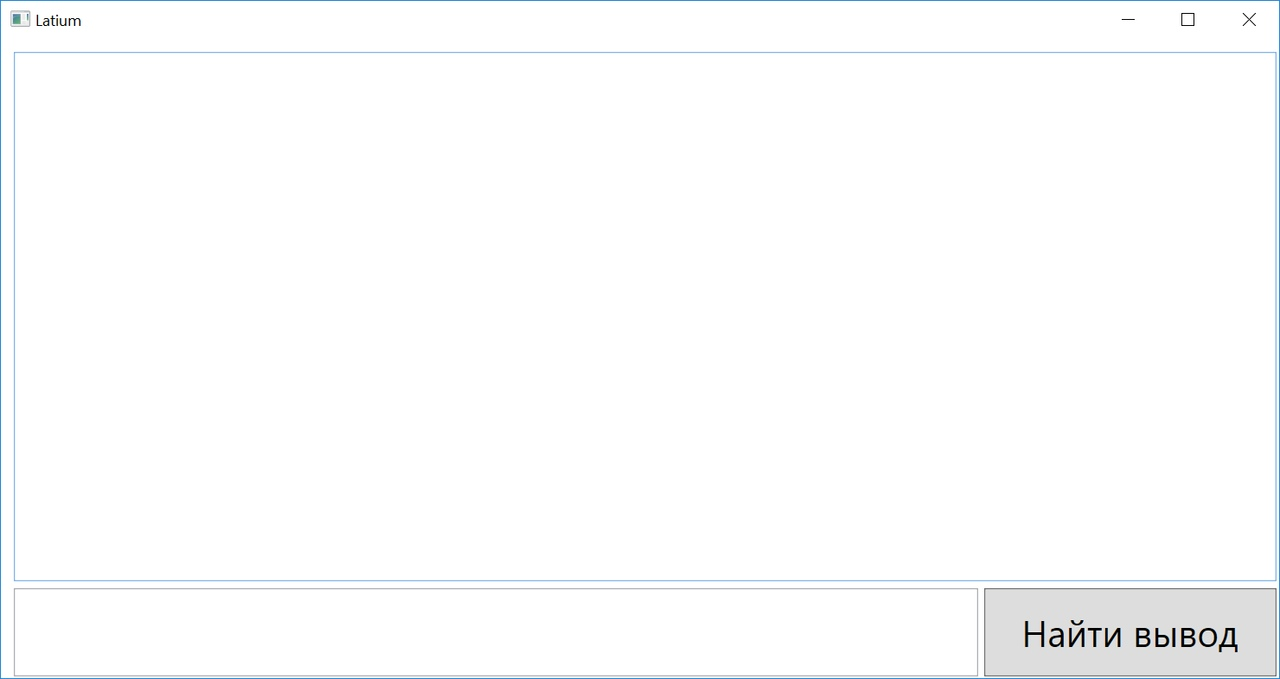
\includegraphics[width=0.8\linewidth]{emptyWindow}
		\end{center}
		\caption{Интерфейс программы «Latium»}
		\label{emptyWindow}
	\end{figure}

	Центральное поле предназначено для вывода на экран результата работы программы - вывода формулы. Поле расположенное внизу - для ввода формулы. Если будет введена не формула, то появится окно, информирующее о том, что введённая строка не является формулой. А  по тексту на кнопке ясно, что она запускает выполнение алгоритма поиска вывода.
	
	Отдельно стоит сказать про ввод формул (см. рисунок \ref{exmpEnter}). Для этого был написан класс PropositionalCalculusTextBox, который является наследником класса TextBox. Этот класс имеет ряд отличий от базового класса:
	\begin{itemize}
		\item Если справа от буквы начать вводить число, то цифры образуют нижний индекс этой буквы.
		\item Если ввести символ $ - $, то в поле ввода появится символ $\lnot$.
		\item Если ввести символ $ > $, то в поле ввода появится символ $\to$.
		\item Если ввести символ $ | $, то в поле ввода появится символ $\lor$.
	\end{itemize}

	\begin{figure}[h]
		\begin{center}
			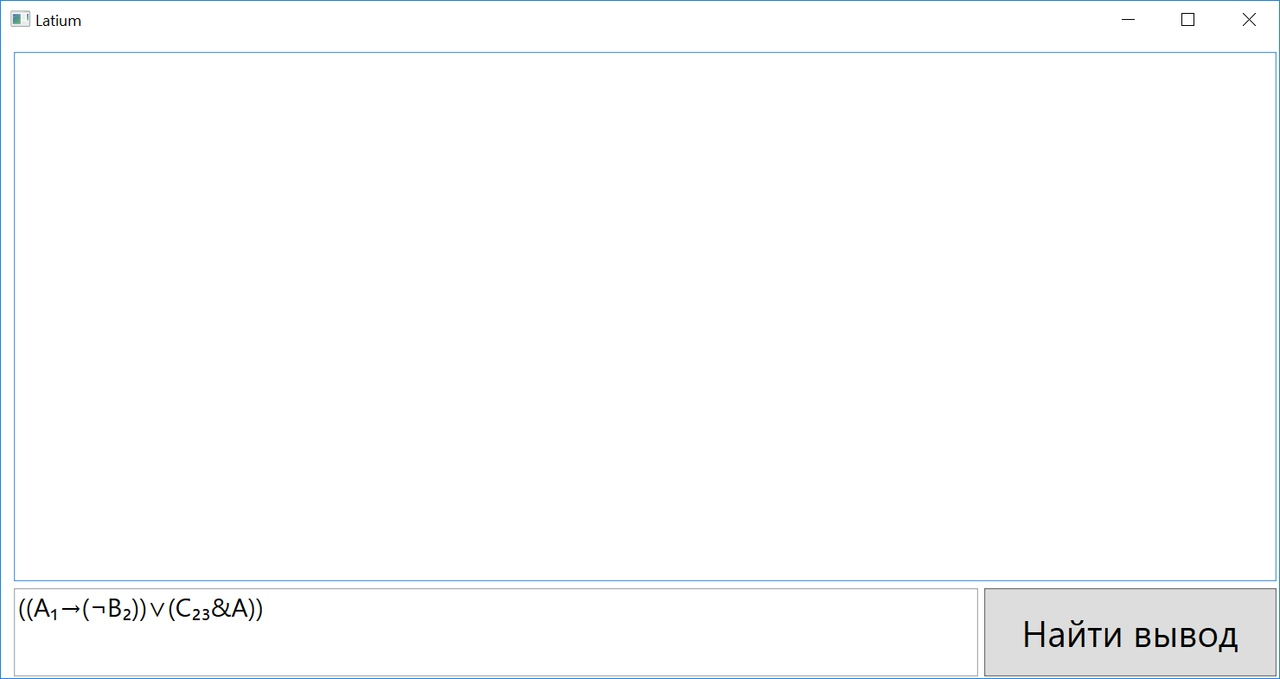
\includegraphics[width=0.8\linewidth]{exmpEnter}
		\end{center}
		\caption{Демонстрация работы ввода}
		\label{exmpEnter}
	\end{figure}
		
	\subsection{Распознавание формулы}
	В первую очередь, нужно решить задачу распознавания формулы: \textit{является ли данная строка формулой Исчисления Высказываний?}
	
	Для решения этой задачи применялся тот же подход, что используется, например, для решения задачи распознавания арифметических выражений:
	\begin{enumerate}
		\item Разбиваем данную строку на токены, то есть отделяем пропозициональные переменные, пропозициональные связки и технические символы друг от друга.
		\item Проверяем расположение пропозициональных связок в строке, например, отрицание должно стоять только перед пропозициональной переменной или левой скобкой.
		\item И наконец, по токенам строится, так называемая, обратная польская запись формулы, в ходе построения которой проверяется баланс скобок в строке.
	\end{enumerate} 
	Если все перечисленные шаги выполняются успешно, без ошибок, то данная на вход строка является формулой Исчисления Высказываний, иначе - не является.
	
	В программе распознавание формулы представлено в конструкторе класса FormulaRpn, а методы Tokenize, CheckTokensOrder и TokensToRpn этого класса - это описанные выше пункты соответственно.
	
	
	\subsection{Способ представления формулы}
	После того, как удалось распознать формулу, естественно возникает другой вопрос: \textit{как представить формулу в памяти компьютера?}
	
	Выше было описано распознавание формул, в ходе которого получалась обратная польская запись этой формулы. Однако можно пойти дальше, а именно, пусть каждая формула в памяти компьютера - это
	\begin{itemize}
		\item либо массив из одного элемента - пропозициональной переменной, если формула является элементарной формулой,
		\item либо массив из двух элементов - формула $\mathcal{B}$ и символ отрицания, если формула имеет вид $ \left(\lnot \mathcal{B}\right)  $,
		\item либо массив из трёх элементов - формула $\mathcal{B}$, формула $\mathcal{C}$ и пропозициональная связка, если формула имеет вид $\left( \mathcal{B} \lor \mathcal{C} \right)$, или $
		\left( \mathcal{B} \& \mathcal{C}\right)$, или $  
		\left( \mathcal{B} \to \mathcal{C}\right)$.
	\end{itemize}
	Такая структура, \textit{во-первых}, позволяет быстро определять какой же вид имеет формула, что полезно, например, при сравнении формул. \textit{Во-вторых}, позволяет быстро получить подформулы, что необходимо при применении правила \textbf{\textit{MP}}. \textit{В-третьих}, позволяет сократить расходы памяти, например, при выполнении замены переменных в формуле необходимо лишь заменить ссылки на переменные ссылками на формулы, на которые происходит замена. Возможно, достоинства такого представления этим не исчерпываются. 
	
	В программе такая форма представления формулы реализована в классах FormulaRpn и Formula, а метод MinimizeRpn класса FormulaRpn по обратной польской записи формулы строит такую структуру.
	
	\subsection{Распознавание аксиом}
	 В описании алгоритма \ref{alg1} есть проверка условия: можно ли добавить формулу в конец вывода. По определению, если формула является аксиомой, то её можно добавить в вывод. Так и возникает задача распознавания аксиом: \textit{является ли данная формула аксиомой Исчисления Высказываний?}
	 
	 Для решения этой задачи был написан класс FormulaMatcher, метод Match которого умеет сопоставлять формулу с шаблоном, считая переменные в шаблоне некоторыми формулами. Например, первая аксиома Исчисления Высказываний соответствует шаблону $ \left( A \to B \right)  $, но не соответствует шаблону $ \left( A \to A \right)  $ .
	 
	 Таким образом, чтобы узнать является ли данная формула аксиомой, необходимо попытаться эту формулу сопоставить с каждой из формул из определения \ref{axiomdef} как с шаблоном. Если формула соответствует одной из этих формул, то она является аксиомой.
	
	\subsection{Способ представления вывода}
	Кроме аксиом, в конец вывода также можно добавить формулу, которая может быть получена по правилу \textbf{\textit{MP}} из формул вывода. Метод FindMpPair класса Inference по формуле как раз и пытается найти для формулы её «\textbf{\textit{MP}} пару». Для того, чтобы ускорить этот поиск, вывод представлен не в виде списка формул, а ввиде словаря с ключами типа формула и со значениями типа целое число - порядковый номер формулы в выводе. Такое представление также позволяет не допустить повторного добавления формулы в вывод, что, очевидно, уменьшает его, а значит поиск по выводу становится быстрее.
	
	Распознавать аксиомы и находить «\textbf{\textit{MP}} пару» - это необходимые и достаточные методы для реализации процедуры добавления формулы в конец вывода (см. метод Push класса Inference).
	
	\subsection{Упрощение вывода}
	В результате работы алгоритма \ref{alg1} в вывод добавляется большое количество аксиом, однако не все из них необходимы для вывода итоговой формулы, то есть можно удалить некоторые формулы из полученной последовательности формул, при этом она не перестанет быть выводом. Так и возникла задача упрощения (сокращения) вывода, которую решает алгоритм \ref{alg2}.  
	
	\begin{algorithm}
	\caption{сокращения вывода формулы Исчисления Высказываний}\label{alg2}
		\begin{algorithmic}[1]
			\State $\mathcal{D}$ - исходный вывод, $\mathcal{D}'$ - новый пустой вывод	
			\State $ \mathcal{A} $ - последняя формула вывода $\mathcal{D}$
			\State \Call{AddFormula}{$ \mathcal{A} $}
			\Procedure{AddFormula}{формула $ \mathcal{A} $}
			\If{$ \mathcal{A} $ - не аксиома}	
			\State 
			\parbox[t]{\dimexpr\linewidth-\algorithmicindent}{ $ \mathcal{A} $ получена из формул $ \mathcal{B} $ и $ \mathcal{C} $ по правилу \textit{\textbf{MP}},\newline которые располагаются левее формулы $\mathcal{A}$ в выводе $\mathcal{D}$ }
			\State \Call{AddFormula}{$ \mathcal{B} $}
			\State \Call{AddFormula}{$ \mathcal{C} $}
			\EndIf	
			\State добавить $ \mathcal{A} $ в конец вывода $\mathcal{D}'$	
			\EndProcedure
		\end{algorithmic}
	\end{algorithm}
	По завершении работы алгоритма $\mathcal{D}'$ - сокращенный вывод.
	Реализован этот алгоритм был как метод Minimize класса Inference.
	
	\subsection{Реализаций алгоритма \ref{alg1}}
	Ранее было выдвинуто предположение, что реализация алгоритма \ref{alg1} «в лоб» не самая лучшая идея. Так и получилось: программа зависала на самых простых формулах. Для решения этой проблемы необходимо «ускорить» алгоритм. 
	
	Заметим, что может возникнуть ситуация, когда необходимые для вывода формулы уже сгенерированы, однако сам процесс генерации ещё не завершён. Поэтому предлагается процессы генерации формул и их добавления в конец вывода выполнять в разных потоках, то есть воспользоваться методами многопоточного программирования языка C\#, о которых можно узнать, например, из книги \cite{YakimovaYaP2}. И замена переменных в аксиомах тоже может происходит в разных потоках. Таким образом, необязательно дожидаться окончания очередной итерации цикла генерации аксиом, а как только вывод будет построен, так сразу завершить работу программы.
	
	Реализация алгоритма \ref{alg1} с использованием методов многопоточного программирования представлена в классе InferenceFinder.
	
	\subsection{Результаты полученные программой «Latium»}
	Итак, программа написана и отлажена, а значит можно переходить к поиску выводов формул Исчисления Высказываний.
	
	Для начала найдём вывод для формулы 
	$ \left(A_{1} \to \left( B_{1} \to A_{1} \right)  \right), $
	которая, очевидно, является аксиомой. Программа определила, что эта формула является аксиомой и вывела вывод состоящий из одной формулы (см. рисунок \ref{ex1}).
	\begin{figure}[h]
		\begin{center}
			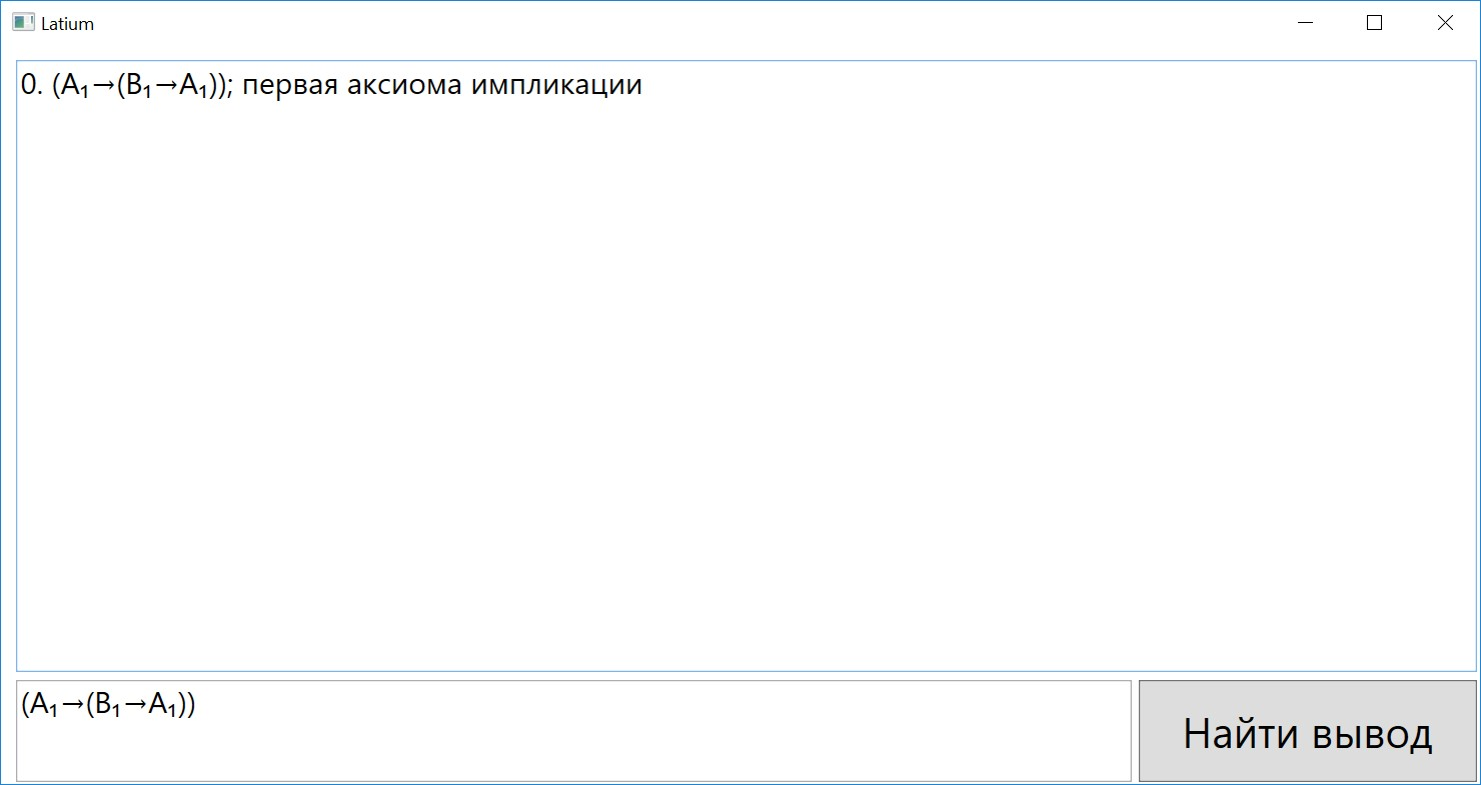
\includegraphics[width=0.8\linewidth]{ex1}
		\end{center}
		\caption{Вывод формулы $ \left(A_{1} \to \left( B_{1} \to A_{1} \right)  \right), $}
		\label{ex1}
	\end{figure}

	Теперь введём формулу 
	$ \left(A \to A\right)$. В некоторых книгах эта формула является первой формулой, для которой приводится вывод. Программа нашла вывод идентичный выводу этой формулы в книге \cite{DurnevML} (см. рисунок \ref{ex2}).
	\begin{figure}[h]
		\begin{center}
			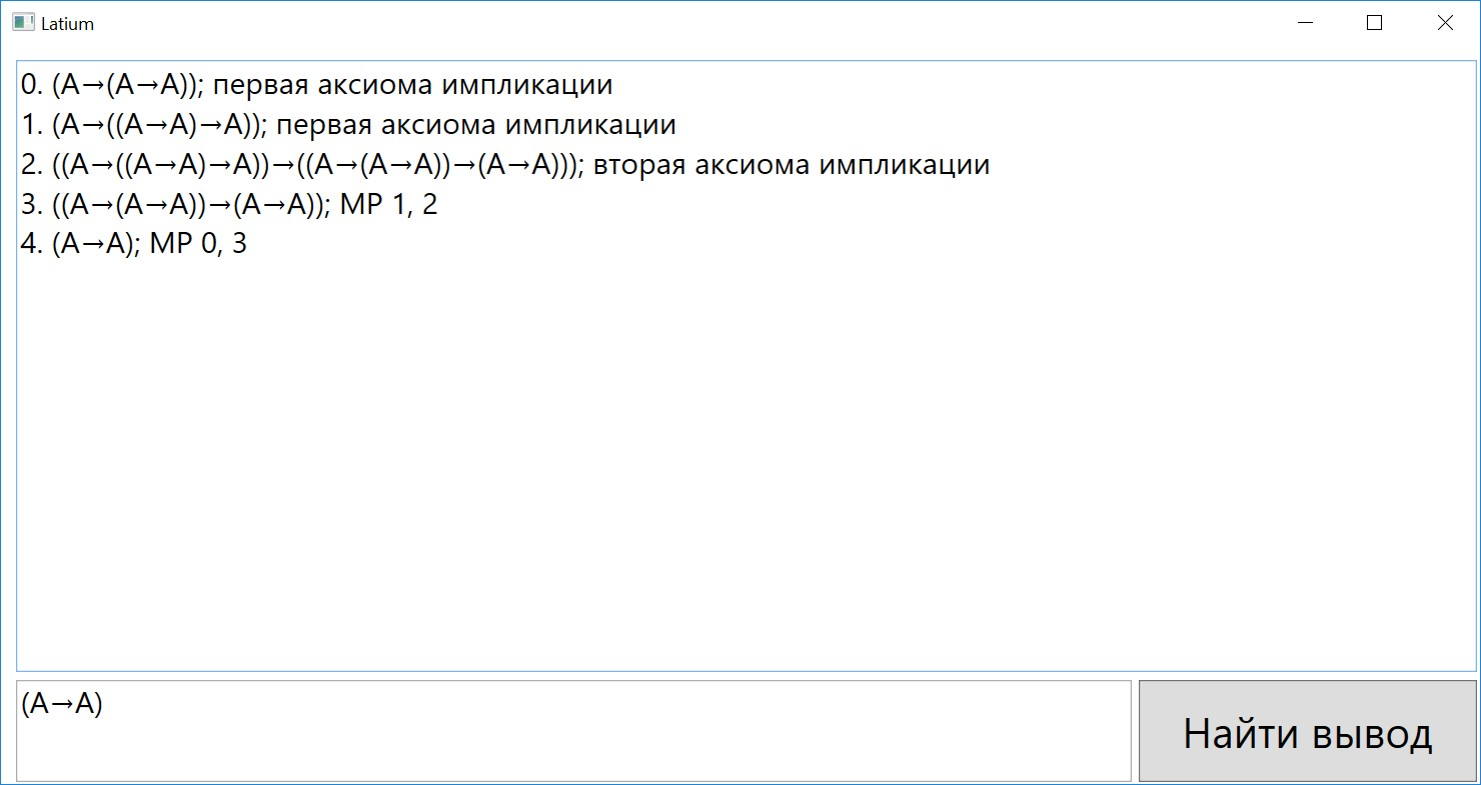
\includegraphics[width=0.8\linewidth]{ex2}
		\end{center}
		\caption{Вывод формулы $ \left(A \to A\right), $}
		\label{ex2}
	\end{figure}

	Рассмотрим формулу $\left( \left( A_{1} \lor A_{1}\right) \to A_{1}\right)  $. Оказалось, что программа «Latium» от запуска к запуску может выводить разные выводы, что и произошло в случае рассматриваемой формулы (см рисунки \ref{ex3.1}, \ref{ex3.2} и \ref{ex3.3}). Это объяснить можно тем, что операционная система во время разных запусков может давать потокам разные интервалы времени, от чего формулы могут генерироваться, а значит и добавляться в вывод, в разном порядке от запуска к запуску. Для усиления этого эффекта формулы при подстановке в аксиомы берутся в случайном порядке (используется стандартный класс Random, генерирующий псевдослучайную последовательность).
	
	Первый вывод формулы $\left( \left( A_{1} \lor A_{1}\right) \to A_{1}\right)  $(рисунок \ref{ex3.1}) можно найти в книгах, а вот два оставшихся вывода (рисунки \ref{ex3.2} и \ref{ex3.3}) являются совершенно новыми.  
	
	\begin{figure}[h]
		\begin{center}
			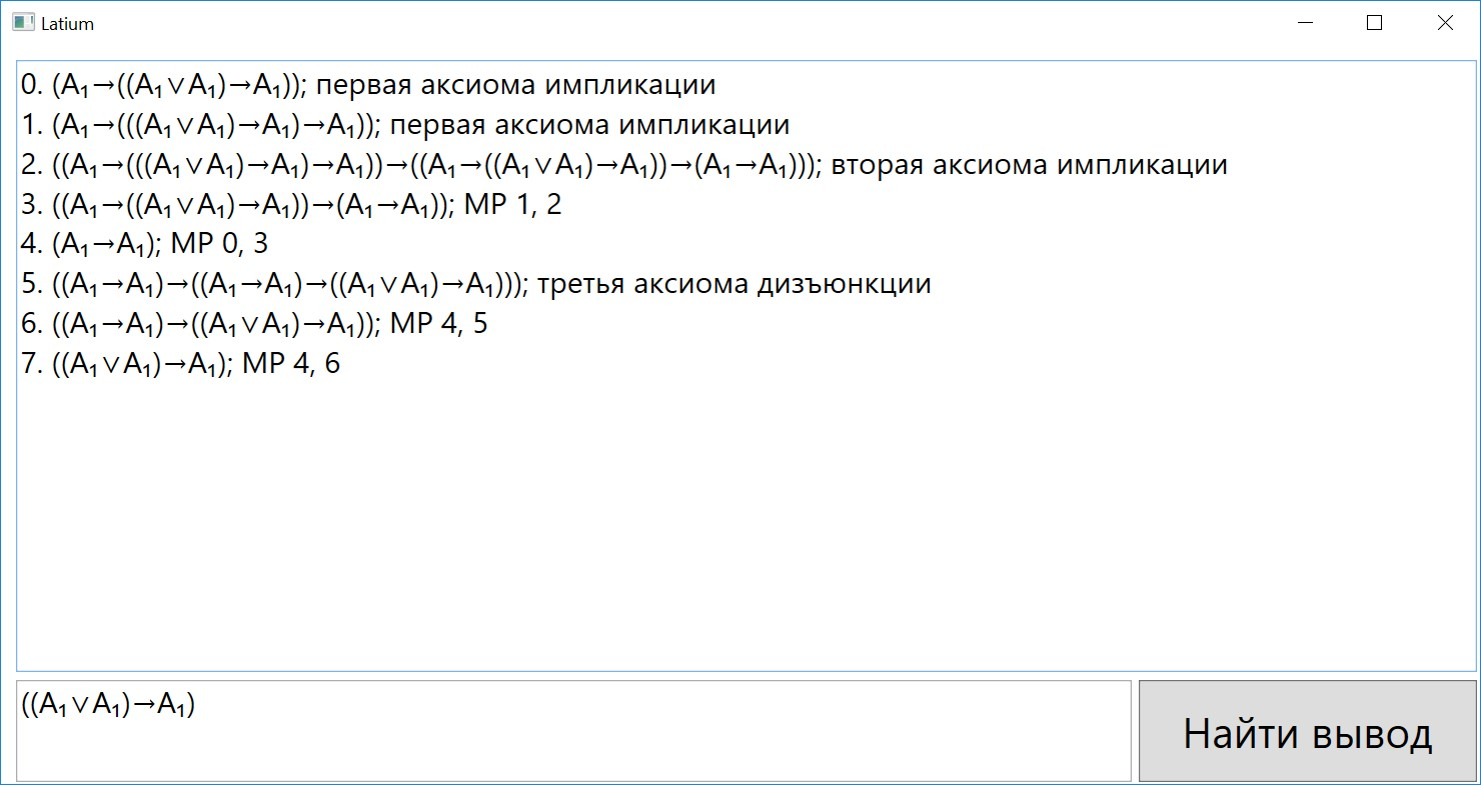
\includegraphics[width=0.8\linewidth]{ex31}
		\end{center}
		\caption{Первый вывод формулы $\left( \left( A_{1} \lor A_{1}\right) \to A_{1}\right)  $}
		\label{ex3.1}
	\end{figure}

	\begin{figure}[h]
		\begin{center}
			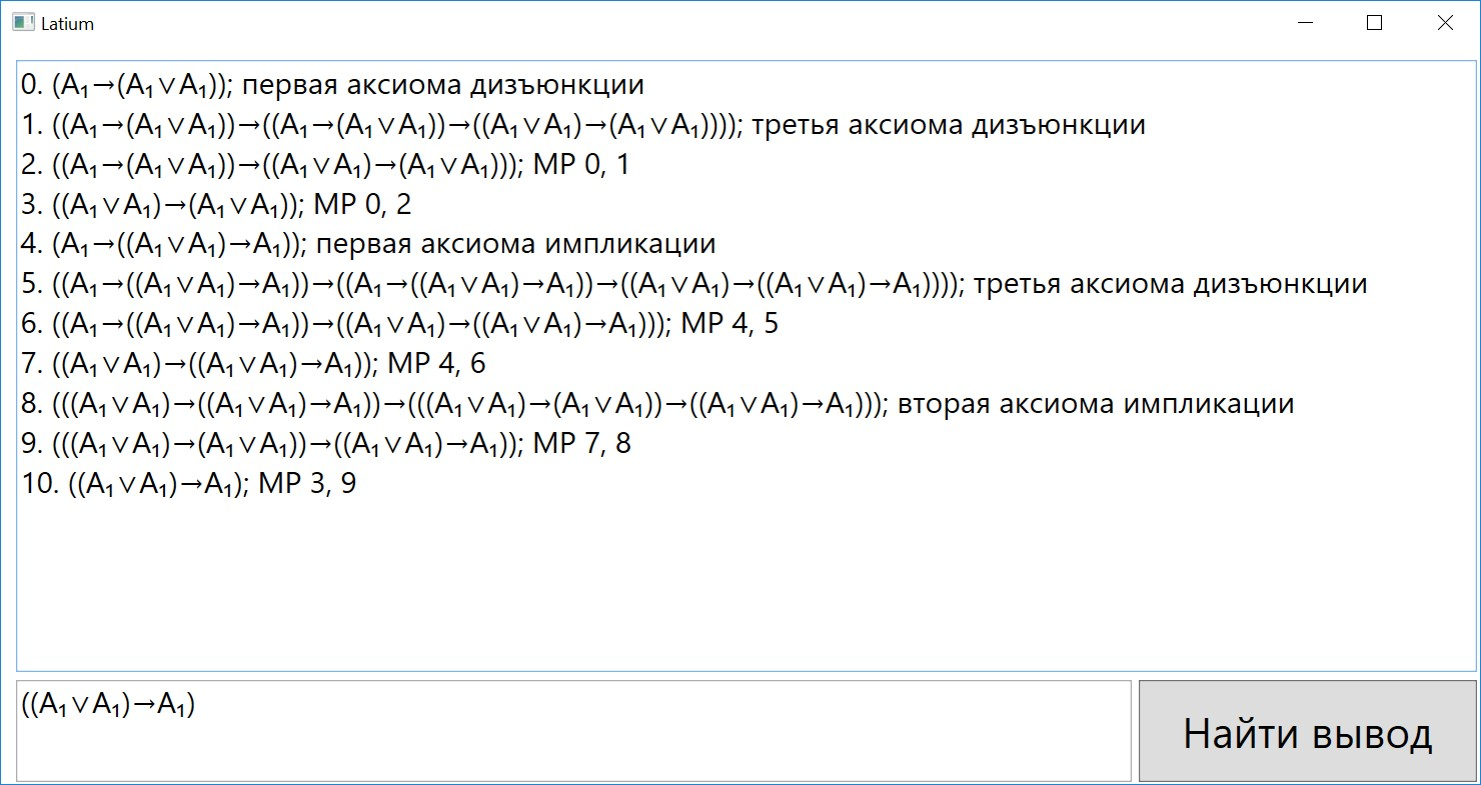
\includegraphics[width=0.8\linewidth]{ex32}
		\end{center}
		\caption{Второй вывод формулы $\left( \left( A_{1} \lor A_{1}\right) \to A_{1}\right)  $}
		\label{ex3.2}
	\end{figure}

	\begin{figure}[h]
		\begin{center}
			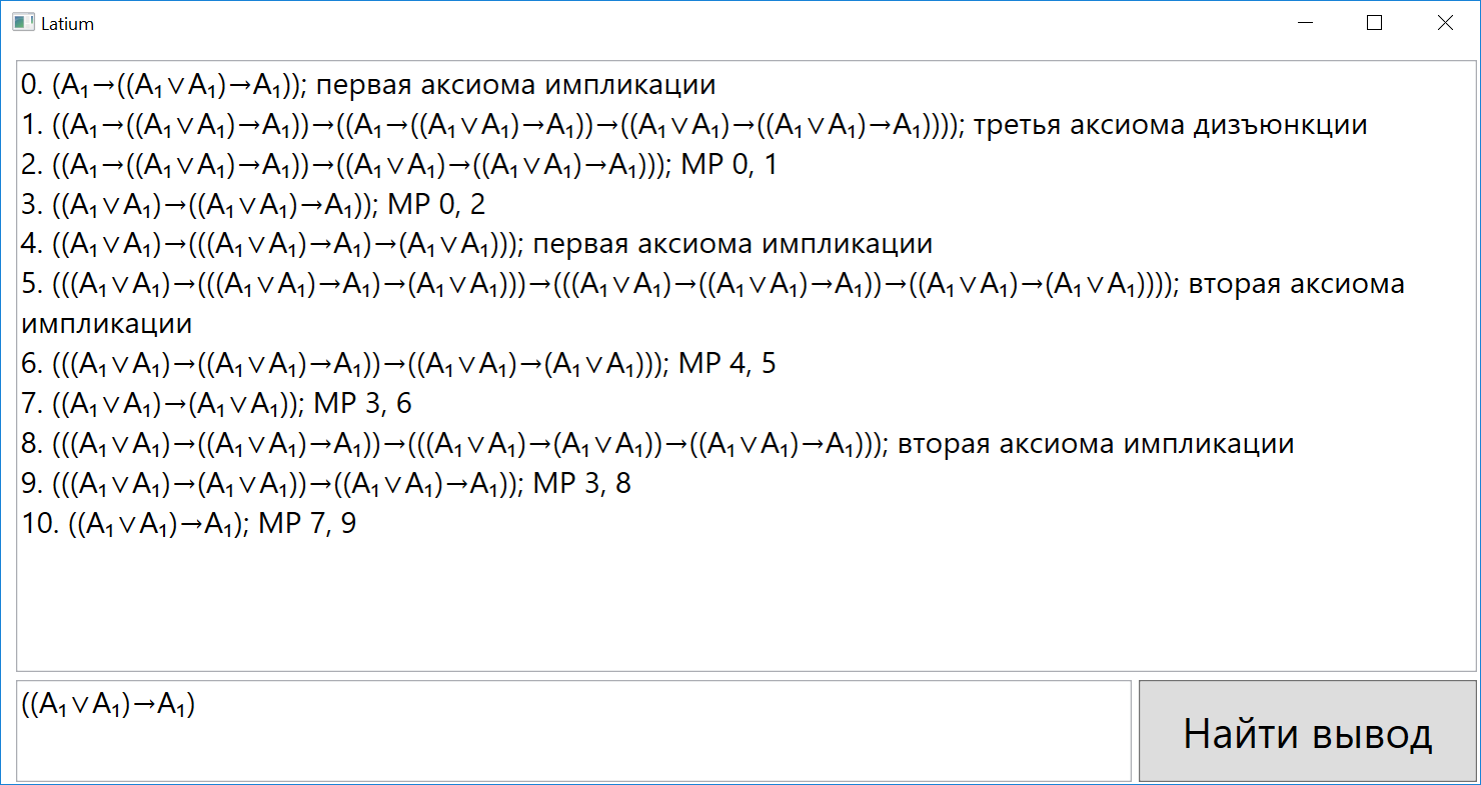
\includegraphics[width=0.8\linewidth]{ex33}
		\end{center}
		\caption{Третий вывод формулы $\left( \left( A_{1} \lor A_{1}\right) \to A_{1}\right)  $}
		\label{ex3.3}
	\end{figure}
	
	\section*{Заключение}
	\addcontentsline{toc}{section}{Заключение}
	Таким образом цель работы достигнута: написана и отлажена компьютерная программа «Latium», которая ищет вывод введённой с клавиатуры формулы Исчисления Высказываний. В этой программе реализовано распознавание формул Исчисления Высказываний, а для представления формулы в компьютере реализована необычная структура данных, основанная на идее обратной польской записи. Также разработан алгоритм \ref{alg1}, который строит вывод формулы, а также реализован алгоритм \ref{alg2}, который упрощает найденный вывод. Написан модифицированный TextBox, облегчающий ввод формул с клавиатуры. И наконец удалось получить выводы для трёх формул, при этом для формулы  $\left( \left( A_{1} \lor A_{1}\right) \to A_{1}\right)  $ были найдены три вывода, два из которых являются совершенно новыми.
	
	В следующем учебном году планируется работа в этом же направлении, а именно решение задач математической логики с применением компьютеров, либо решение задач информатики с применением математической логики. Например, можно продолжить работу в одном из следующих направлений:
	\begin{itemize}
		\item Поиск вывода в Исчислении Предикатов
		\item Поиск вывода в Исчислении Секвенций
		\item Изучение и реализация алгоритма Тарского
		\item Доказательство теорем в формальных системах, например, аксиоматика действительных чисел или аксиоматика арифметики Пеано
		\item Формальная верификация
		
		
	\end{itemize}
	
	\begin{thebibliography}{3}
		\bibitem{DurnevML}
		Дурнев, В.Г. Элементы теории множеств и математической логики: учеб. пособие / В. Г. Дурнев; Яросл. гос. ун-т. им. П. Г. Демидова. – Ярославль, 2009. 457 с. 
		\bibitem{YakimovaYaP2}
		Якимова, О. П. Языки программирования. Ч.2: лабораторный практикум / О. П. Якимова, И. М. Якимов, В. Л. Дольников; Яросл. гос. ун-т им. П. Г. Демидова. – Ярославль : ЯрГУ, 2012 – 56 с.  
	\end{thebibliography}
	\addcontentsline{toc}{section}{\refname}
	
	\section*{Приложение А}
	\addcontentsline{toc}{section}{Приложение А}
	Ссылка на репозиторий с исходным кодом программы «Latium» на GitHub: https://github.com/romarioGI/Latium.
	
	~
	
	Навигация по репозиторию:
	\begin{itemize}
		\item класс \textbf{Inference} (вывод) - \newline Latium/Latium/PropositionalCalculusLibrary/Inference.cs
		
		\item класс \textbf{Formula} (формула) - \newline
		Latium/Latium/PropositionLibrary/Formula.cs
		
		\item класс \textbf{FormulaRpn} (обратная польская запись формулы) - \newline
		Latium/Latium/PropositionLibrary/FormulaRpn.cs
		
		\item класс \textbf{FormulaMatcher} («сопоставитель» формул) - \newline
		Latium/Latium/PropositionLibrary/FormulaMatcher.cs
		
		\item класс \textbf{PropositionalCalculusTextBox} (ввод формулы) - \newline
		Latium/Latium/PropositionalCalculusTextBox/PropositionalCalculusTextBox.cs
		
		\item класс \textbf{InferenceFinder} (реализация алгоритма \ref{alg1}) - \newline
		Latium/Latium/PropositionalCalculusInferenceFinder/InferenceFinder.cs
		
	\end{itemize}
	
\end{document}